\section{Method and Data} 
\label{sec:method}
From a holistic view of research method (Figure~\ref{fig:System structure}), it
consists several relational parts of the dataset import,dataset Processing, and machine model training for topic clustering

In dataset import process, since the dataset is un-hydrated, we needed
to “hydrate” the data by building a process that will fetch the tweet content
by querying with the Tweet ID. After hydrating, the data are saved in a local
storage, and by using Tweets API the data are completed to be analyzed and
stored in the Elasticsearch server. 
\begin{figure}[h]
\centering
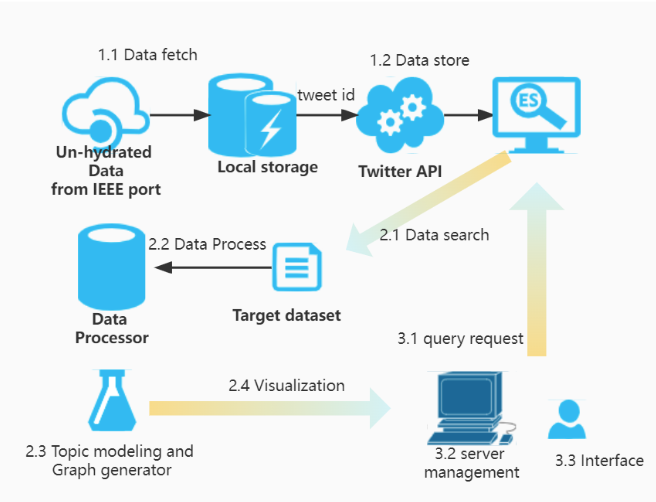
\includegraphics[width=0.5\textwidth]{imgs/framework/framework.png}
\caption{System structure}
\label{fig:System structure}
\end{figure}
In dataset processing step, after importing data into Elasticsearch server in
batches, we choose a research scope and we get the target dataset from
Elasticsearch. By doing spatial query and filtering task, the target dataset
can be visualized into a map. Furthermore, after processing the data by using
techniques such as the regex filtering, tokenization and tagging, and
removing stop words, it is possible to apply a topic clustering model to get topics.


\subsection{Tweet Data Collection and Processing}
\subsubsection{Tweet Data Collection process}
The dataset we used is CORONAVIRUS (COVID-19) GEO-TAGGED TWEETS DATASET form
IEEE DataPort. Due to the tweets spreading policy. We can't access the
completed tweets content directly.  Thus. We use a transfer program named
Twarc to batch fetch tweets in the dataset. Twarc is a python package
that used to export tweets automatically.  The main principle is that Twarc
will make use of the registration information from twitter developer platform
and get the permission from Twitter. Then Twitter can monitor the whole
process of getting tweets. This way is completely legal and doesn't violate
the privacy protocols set by Twitter. But it also cause some issues. If the
tweets account is banned or the permission has been changed, we can't access
the content anymore. Normally Twitter doesn't send any warning message but
change the content of tweets to a prompt message. So some filtering process
is necessary to ensure that the data set is not contaminated with irrelevant
information. 

We collect data from March 2020 to March 2022. These data comes form hundreds
of single CSV files, Since they are stored by date. So a batch process is
necessary to import from these files. After that we store all of these data
to Elasticsearch, in order to facilitate subsequent steps to call on demand. 

\subsubsection{Tweet Data structure}
The original data contains tweets ID and sentiment score calculated by
database publisher Figure~\ref{fig:Tweet dataset}. We use tweets ID to
request twitter API in batch and get completed information, including
content, UTC time, geographic location. All of these information are fully
imported into the server after splicing with sentiment score.  In this
process, we will transfer the longitude and latitude to the geometry, then we
can apply some spatial operator to handle them. Time format is another point.
In this way, we transfer all the time appearing in our project to UTC format.
Then all filtering of time will be consistent. 
\begin{figure}[h]
\centering
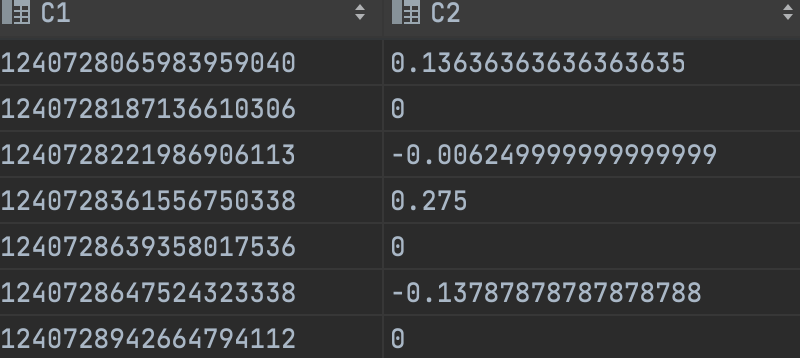
\includegraphics[width=0.5\textwidth]{imgs/row_tweets.png}
\caption{Tweet dataset structure}
\label{fig:Tweet dataset}
\end{figure}
\subsubsection{Tweet Data Pre-processing Method}
The pre-processing process includes regex filtering, tokenization and tagging,
removal of stop words (Figure~\ref{fig:Tokenization and tag}). Regex
filtering process used to delete some proper noun or URL. We set different filtering rules according to the task goals and model requirements. For example, deleting all emojis, filtering misspelled words based on word list.  

Tokenization and tag are important to our project. We use nltk package to
process the sentence in the tweets and decompose the content into single
words. Then we can filter for parts of speech and get more reasonable
results. 
\begin{figure}[h]
\centering
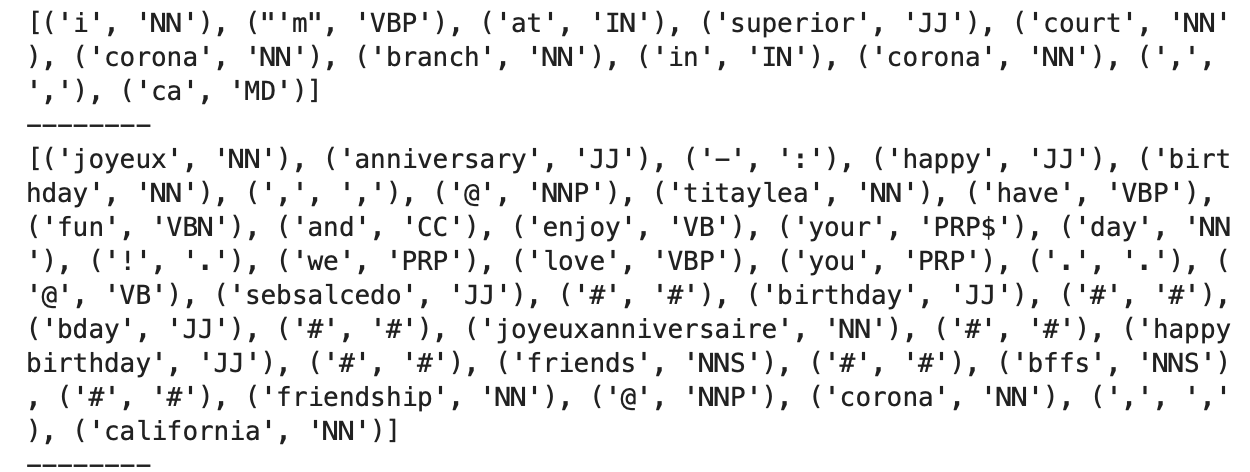
\includegraphics[width=0.5\textwidth]{imgs/tokenization.png}
\caption{Tokenization and tag}
\label{fig:Tokenization and tag}
\end{figure}
The purpose of removal of stopwords is to avoid distractions from common words
on the topic. The nltk package provide a library of stopwords and we can set
our own list of common words based on the theme. It's an important step to
get good performance of machine learning models and we can adjust it to fit
the current strategy we used.

\subsection{Sentence vector generation}
We propose to use a LDA-BERT based method to generate vector for each tweet. First, we break down tweets into body and hashtags. For the body part, we tokenize the sentences and train them with BERT. Then we get vectors which contains hundreds of dimensions. For the hashtags part, we apply LDA on them and generate vectors of corresponding dimensions according to the number of topics to be divided into. To combine the information form two resource, we use autoencoder to compress combined vector.

\begin{figure}[h]
\centering
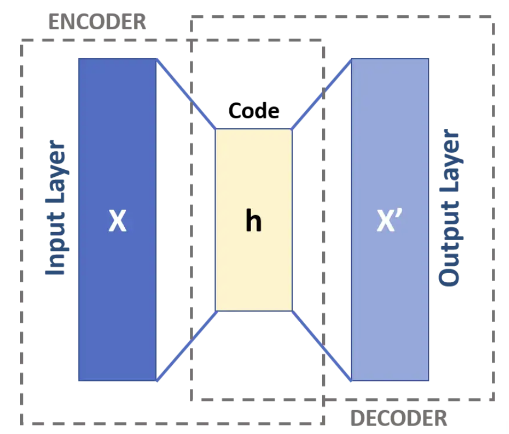
\includegraphics[width=0.5\textwidth]{imgs/framework/autoencoder.png}
\caption{structure of autoencoder}
\label{fig:autoencoder}
\end{figure}

By this method, we succeed in reducing the dimensionality of the resulting vector while preserving topic features.

\subsection{Topic Clustering}
We use Time Series KMeans to do the clustering. Because each tweet is attached with publish time, we need to consider its temporal correlation while clustering. 

\subsection{Visualization}
\subsubsection{Wordcloud}
Wordcloud is a graph to show the high frequency words. After clustering, we get labels which indicate which cluster the current tweet belongs to. Then we get all word lists under the same cluster and concat them. Finially the wordcloud will show higher frequency words in bigger font.
\subsubsection{Centroid sentence}
To study topic relevance, we calculate the cosine similarity between every tweet and cluster centroid point and pick up the nearest tweet as the most representative tweet.  
\subsubsection{Storyline}
To generate a graph showing all topic relationships, we caculate the similarity between all the topic pair. Then sort the calculation results from high to low. Based on it, we set a threshold of edge. An edge will be generated between all topic pairs whose similarity is greater than the threshold. Finally we import the point and edge information into Graphviz and get a graph.(Fig~\ref{fig:storyline for lda_bert}) 
